\documentclass{article}
\usepackage[utf8]{inputenc}
\usepackage[a4paper, total={7in, 10in}]{geometry}
\usepackage{graphicx}
\graphicspath{ {./pic/} }
\title{Sections and Chapters}
\author{Gubert Farnsworth}
\date{ }
  
\begin{document}
  
\maketitle

\tableofcontents

\section{Introduction}
   
This is the first section.

\subsection{Introduction}
Árvíztűrő tükörfúrógép.

Lorem  ipsum  dolor  sit  amet,  consectetuer  adipiscing  
elit.   Etiam  lobortisfacilisis sem.  Nullam nec mi et 
neque pharetra sollicitudin.  Praesent imperdietmi nec ante. 
Donec ullamcorper, felis non sodales...

\begin{figure}[h]
    \centering
    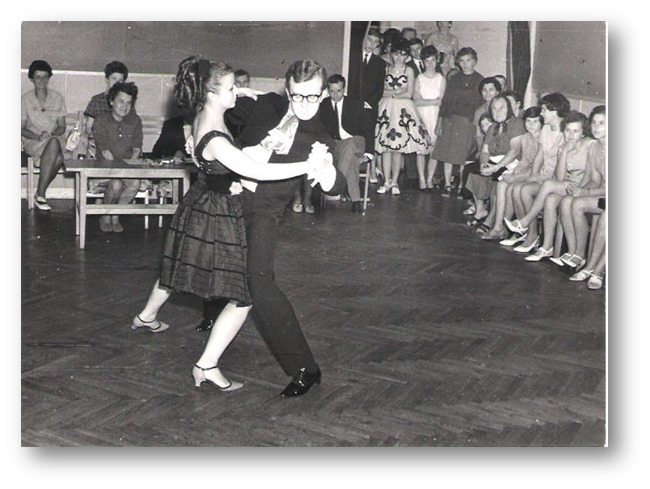
\includegraphics[scale=0.6]{joskabacsi}
    \caption{a nice plot}
    \label{fig:mesh1}
\end{figure}

\addcontentsline{toc}{section}{Unnumbered Section}
\section*{Unnumbered Section}

The well known Pythagorean theorem \(x^2 + y^2 = z^2\) was 
proved to be invalid for other exponents. 
Meaning the next equation has no integer solutions:

\[ x^n + y^n = z^n \]

The mass-energy equivalence is described by the famous equation

\[E=mc^2\]

discovered in 1905 by Albert Einstein. 
In natural units ($c$ = 1), the formula expresses the identity

\begin{equation}
E=m
\end{equation}

Greek letters: \(\alpha \beta \gamma \rho \sigma \delta \epsilon \)

\begin{center}
\begin{tabular}{||c c c c||} 
\hline
Col1 & Col2 & Col2 & Col3 \\ [0.5ex] 
\hline\hline
1 & 6 & 87837 & 787 \\ 
\hline
2 & 7 & 78 & 5415 \\
\hline
3 & 545 & 778 & 7507 \\
\hline
4 & 545 & 18744 & 7560 \\
\hline
5 & 88 & 788 & 6344 \\ [1ex] 
\hline
\end{tabular}
\end{center}

\section{Second Section}
       
Lorem ipsum dolor sit amet, consectetuer adipiscing elit.  
Etiam lobortis facilisissem.  Nullam nec mi et neque pharetra 
sollicitudin.  Praesent imperdiet mi necante...

\listoffigures

\end{document}